\documentclass[11pt,a4paper]{article}
\usepackage[margin=2.5cm]{geometry}
\usepackage{booktabs,graphicx,amsmath,amssymb}
\usepackage[hidelinks]{hyperref}
\usepackage{natbib}
\usepackage{caption}
\captionsetup{font=small}
\title{Multi-Timeframe Key Levels:\\ A Pre-Registered Replication and Null Result}
\author{Key-Level Research Project}
\date{2026-11-02 14:34 UTC}
\begin{document}
\maketitle
\begin{abstract}
We test a widely circulated multi-timeframe key-level strategy on eight liquid instruments over 2012--2025. On the 2012--2019 development sample (7,891 trades), the gross mean return is -0.015R per trade and the net mean return is -0.205R after a conservative half-spread-plus-slippage assumption (net annualised Sharpe -3.52). All 18 pre-registered parameter combinations have a negative net Sharpe ratio. On the sealed 2023--2025 holdout (3,155 trades), the net mean return is -0.166R and the net annualised Sharpe is -2.79; the pre-registered success criterion is not met. In a separate event study of executed signals, the strict hold rate (no close through the level over the next 96 bars) was 15.5\%, and price reached +1R before -1R in 49.2\% of cases. Even the weaker +1R measure is far below the 90\% success rate claimed by practitioners. The evidence rejects the strategy as operationalised here: the gross mean return is slightly negative, the result is stable across a pre-registered parameter grid, and the sealed holdout does not reverse the conclusion.
\end{abstract}
\noindent\textbf{Keywords:} technical analysis; support and resistance; foreign exchange; intraday; backtest overfitting; replication

\section{Introduction}
Technical analysis remains widely used in foreign exchange and futures markets, yet the profitability of simple chart patterns after realistic costs and data-snooping corrections is contested \citep{brock1992simple,lo2000foundations,menkhoff2007obstinate,osler2003currency}. This paper studies a specific and widely taught workflow: mark monthly, weekly, and daily support/resistance from candle bodies; determine the trend on the 4-hour chart; wait for a 15-minute rejection at a level; enter in the trend direction with a stop beyond the level and a target at the next level. The practitioner claim is that the level holds roughly 90\% of the time. We translate the workflow into deterministic rules, freeze the rules before opening a sealed 2023--2025 holdout, and report the result whatever its sign.
Our contribution is a well-powered negative result with three features that are often missing from practitioner replications: (i) intraday data from an independent vendor over 2012--2025, (ii) a pre-registered parameter grid and sealed holdout, and (iii) inference that corrects for the selection of the best variant \citep{bailey2014deflated,bailey2017probability,white2000reality,hansen2005test}.
\section{Related literature}
The modern literature on technical trading begins with \citet{brock1992simple}, who documented predictability using simple rules on the Dow, and \citet{sullivan1999data}, who showed that data-snooping can explain much of the apparent profitability. \citet{lo2000foundations} formalised pattern recognition and found some incremental information in chart patterns. In foreign exchange, \citet{osler2003currency} linked the predictive success of technical analysis to the clustering of stop and take-profit orders around round numbers, and \citet{menkhoff2007obstinate} documented the continued use of technical analysis by professionals. More recent work continues to find horizon- and regime-dependent predictability \citep{rink2023predictive,deprez2024bitcoin}. Our design follows the backtesting protocol of \citet{arnott2019backtesting} and the multiple-testing corrections of \citet{harvey2020false}.
\section{Data}
The primary sample is HistData.com Generic ASCII M1 bid bars for eight instruments: EURUSD, GBPUSD, USDJPY, AUDUSD, USDCAD, XAUUSD, SPXUSD, and NSXUSD, from 2012-01-01 to 2025-12-31. M1 bars are resampled into 15-minute, 4-hour, daily, weekly, and monthly bars. No future bar is used before its close. HistData timestamps are treated as fixed UTC-5 without daylight saving, per the vendor specification. The processed sample contains 346,372 EURUSD 15-minute bars, 330,920 XAUUSD bars, and 324,578 SPXUSD bars.
An independent check compares weekly close-to-close returns with Yahoo Finance daily bars. The Yahoo series are not mixed into the historical backtest. The 2026 live shadow uses Yahoo 15-minute bars, whose public window is roughly 59 days, and is descriptive only.
\begin{table}[htbp]\centering\small
\caption{Instrument universe and base round-trip cost assumptions.}
\label{tab:instruments}
\begin{tabular}{llrrr}
\toprule
Instrument & Class & Half-spread & Slippage & Round trip \\
\midrule
EURUSD & fx major & 3e-05 & 2e-05 & 0.0001 \\
GBPUSD & fx major & 4e-05 & 3e-05 & 0.00014 \\
USDJPY & fx major & 0.003 & 0.002 & 0.01 \\
AUDUSD & fx major & 4e-05 & 3e-05 & 0.00014 \\
USDCAD & fx major & 4e-05 & 3e-05 & 0.00014 \\
XAUUSD & metal & 0.15 & 0.1 & 0.5 \\
SPXUSD & equity index & 0.25 & 0.25 & 1 \\
NSXUSD & equity index & 0.5 & 0.5 & 2 \\
\bottomrule
\end{tabular}
\end{table}
\section{Strategy and execution}
Monthly, weekly, and daily pivots are clustered in price with a tolerance of $0.50\times$ ATR14(D1) and become tradable after at least two pivots. A level is a resistance if a 15-minute bar trades through it and closes back below; a support is the mirror case. The 4-hour trend is defined by the last two confirmed swing highs and lows. A trade requires trend agreement, a level touch, two consecutive closes on the rejected side, a directional candle, and a chase of no more than $1\times$ ATR15. Entry is at the next 15-minute open.
The stop is the more conservative of the level plus $0.25\times$ ATR15 and the five-bar extreme plus $0.10\times$ ATR15, capped at $4\times$ ATR15. The target is the nearest opposite active level at least $1R$ away, defaulting to $2R$ and capped at $5R$. Maximum holding period is 96 bars. If the stop and target share a bar, the stop is assumed first. Risk is 0.5\% of equity per trade. Costs are half the quoted spread plus adverse slippage on each side. A gap through the stop fills at the next available open; a gap through the target does not enter the trade.
\begin{table}[htbp]\centering\small
\caption{Frozen base parameters.}
\label{tab:design}
\begin{tabular}{ll}
\toprule
Parameter & Value \\
\midrule
entry timeframe & 15min \\
trend timeframe & 4h \\
level timeframes & ['1D', '1W', '1M'] \\
pivot left & 2 \\
pivot right & 2 \\
trend pivot left & 3 \\
trend pivot right & 3 \\
level price source & body \\
cluster atr & 0.5 \\
min touches & 2 \\
level expiry days & 730 \\
touch lookback & 300 \\
confirmation closes & 2 \\
max chase atr & 1.0 \\
stop buffer atr & 0.25 \\
stop extreme lookback & 5 \\
stop extreme buffer atr & 0.1 \\
max stop atr & 4.0 \\
default rr & 2.0 \\
max rr & 5.0 \\
max hold bars & 96 \\
risk per trade & 0.005 \\
require directional candle & True \\
trend method & swing \\
require trend & True \\
ema length & 200 \\
ema slope bars & 5 \\
\bottomrule
\end{tabular}
\end{table}
\section{Statistical protocol}
The sample is split into development (2012--2019), validation (2020--2022), and a sealed holdout (2023--2025). The base specification is fixed by faithfulness to the transcript, not optimised. The 18-point grid is selected on development only; the winner is evaluated unchanged on validation and holdout. Inference uses the stationary bootstrap \citep{politis1994stationary}, the deflated Sharpe ratio \citep{bailey2014deflated}, the probability of backtest overfitting via CSCV \citep{bailey2017probability}, the White Reality Check \citep{white2000reality}, Hansen's SPA test \citep{hansen2005test}, and Benjamini--Hochberg control of the per-instrument false discovery rate \citep{benjamini1995controlling}. The holdout is opened once, after a SHA-256 code freeze.
\section{Results}
On the development sample the base strategy produced 7,891 trades. Gross mean return was -0.015$R$ per trade and net mean return was -0.205$R$, with net annualised Sharpe -3.52 and maximum drawdown -99.97%. The cost drag was +0.190$R$ per trade.

\begin{table}[htbp]
\centering
\footnotesize
\setlength{\tabcolsep}{4pt}
\caption{Base strategy by sample split.}
\label{tab:splits}
\begin{tabular}{lrrrrr}
\toprule
Metric & Dev 2012--19 & Val 2020--22 & Holdout 2023--25 & Val winner & Holdout winner \\
\midrule
Trades & 7,891 & 3,556 & 3,155 & 1,831 & 1,460 \\
Trading days & 2,087 & 783 & 783 & 783 & 783 \\
Annual return & -62.38\% & -53.72\% & -55.89\% & -39.54\% & -25.05\% \\
Annual volatility & 26.72\% & 30.17\% & 27.91\% & 22.54\% & 19.93\% \\
Net Sharpe & -3.52 & -2.40 & -2.79 & -2.12 & -1.35 \\
Max drawdown & -99.97\% & -91.62\% & -92.45\% & -80.51\% & -59.83\% \\
Win rate & 29.07\% & 30.76\% & 29.38\% & 26.49\% & 27.19\% \\
Mean net R & -0.205 & -0.121 & -0.166 & -0.169 & -0.141 \\
Mean gross R & -0.015 & +0.002 & -0.028 & -0.019 & +0.025 \\
Cost drag & +0.190 & +0.123 & +0.138 & +0.150 & +0.166 \\
Profit factor & 0.747 & 0.838 & 0.789 & 0.795 & 0.831 \\
Stop rate & 65.25\% & 64.26\% & 65.86\% & 69.52\% & 68.22\% \\
Target rate & 18.72\% & 21.46\% & 19.24\% & 18.79\% & 16.51\% \\
\bottomrule
\end{tabular}
\end{table}
Table \ref{tab:grid} reports the full grid. Every combination has a negative net Sharpe. The least-negative variant is grid\_c1.0\_m3\_k3 (Sharpe -2.26), selected only by ranking losses. Figure \ref{fig:grid} shows the same surface graphically.
\begin{table}[htbp]
\centering
\footnotesize
\setlength{\tabcolsep}{4pt}
\caption{Pre-registered parameter grid on the development sample.}
\label{tab:grid}
\begin{tabular}{lrrrrrrr}
\toprule
Variant & Cluster & Touches & Confirms & Trades & Sharpe & Mean net R & Win rate \\
\midrule
grid\_c1.0\_m3\_k3 & 1.00 & 3 & 3 & 3,675 & -2.26 & -0.215 & 25.66\% \\
grid\_c1.0\_m3\_k2 & 1.00 & 3 & 2 & 4,760 & -2.46 & -0.195 & 27.63\% \\
grid\_c1.0\_m2\_k3 & 1.00 & 2 & 3 & 4,494 & -2.61 & -0.218 & 26.10\% \\
grid\_c0.25\_m3\_k3 & 0.25 & 3 & 3 & 5,208 & -2.69 & -0.201 & 28.32\% \\
grid\_c1.0\_m2\_k2 & 1.00 & 2 & 2 & 5,831 & -2.75 & -0.191 & 28.18\% \\
grid\_c0.25\_m3\_k2 & 0.25 & 3 & 2 & 6,774 & -2.78 & -0.173 & 29.88\% \\
grid\_c1.0\_m3\_k1 & 1.00 & 3 & 1 & 7,191 & -2.84 & -0.174 & 29.15\% \\
grid\_c0.5\_m3\_k2 & 0.50 & 3 & 2 & 6,002 & -2.94 & -0.201 & 28.41\% \\
grid\_c0.25\_m3\_k1 & 0.25 & 3 & 1 & 10,071 & -2.98 & -0.156 & 31.30\% \\
grid\_c0.5\_m3\_k3 & 0.50 & 3 & 3 & 4,609 & -3.09 & -0.239 & 26.60\% \\
grid\_c1.0\_m2\_k1 & 1.00 & 2 & 1 & 8,702 & -3.23 & -0.177 & 29.56\% \\
grid\_c0.5\_m3\_k1 & 0.50 & 3 & 1 & 8,922 & -3.33 & -0.189 & 29.44\% \\
grid\_c0.5\_m2\_k2 & 0.50 & 2 & 2 & 7,891 & -3.52 & -0.205 & 29.07\% \\
grid\_c0.25\_m2\_k3 & 0.25 & 2 & 3 & 7,547 & -3.60 & -0.219 & 29.07\% \\
grid\_c0.5\_m2\_k3 & 0.50 & 2 & 3 & 6,073 & -3.62 & -0.242 & 27.27\% \\
grid\_c0.25\_m2\_k2 & 0.25 & 2 & 2 & 9,712 & -3.75 & -0.193 & 30.55\% \\
grid\_c0.25\_m2\_k1 & 0.25 & 2 & 1 & 14,328 & -3.93 & -0.169 & 32.01\% \\
grid\_c0.5\_m2\_k1 & 0.50 & 2 & 1 & 11,709 & -3.98 & -0.191 & 30.23\% \\
\bottomrule
\end{tabular}
\end{table}
\begin{table}[htbp]
\centering
\small
\setlength{\tabcolsep}{4pt}
\caption{Pre-registered ablations on the development sample.}
\label{tab:ablations}
\begin{tabular}{lrrrr}
\toprule
Ablation & Trades & Sharpe & Mean net R & Win rate \\
\midrule
no\_trend & 32,645 & -11.01 & -0.215 & 31.24\% \\
no\_confirmation & 14,088 & -4.52 & -0.214 & 29.15\% \\
no\_directional & 12,217 & -4.69 & -0.247 & 27.51\% \\
ema\_trend & 11,566 & -3.50 & -0.191 & 27.36\% \\
wick\_levels & 7,719 & -2.79 & -0.179 & 29.28\% \\
min\_touches\_3 & 6,002 & -2.94 & -0.201 & 28.41\% \\
cluster\_025 & 9,712 & -3.75 & -0.193 & 30.55\% \\
cluster\_100 & 5,831 & -2.75 & -0.191 & 28.18\% \\
confirmation\_1 & 11,709 & -3.98 & -0.191 & 30.23\% \\
confirmation\_3 & 6,073 & -3.62 & -0.242 & 27.27\% \\
\bottomrule
\end{tabular}
\end{table}
On validation (2020--2022) the base strategy produced 3,556 trades with net mean $R$ -0.121 and net Sharpe -2.40. The development grid winner produced 1,831 trades with net mean $R$ -0.169. The sign did not reverse.
On the sealed holdout (2023--2025) the strategy produced 3,155 trades with net mean $R$ -0.166, net Sharpe -2.79, and maximum drawdown -92.45%. The primary endpoint is not met.
\begin{table}[htbp]
\centering
\small
\setlength{\tabcolsep}{4pt}
\caption{Holdout cost sensitivity.}
\label{tab:costs}
\begin{tabular}{lrrr}
\toprule
Cost multiplier & Trades & Mean net R & Net Sharpe \\
\midrule
0.00x & 3,155 & -0.028 & -0.42 \\
1.00x & 3,155 & -0.166 & -2.79 \\
2.00x & 3,155 & -0.304 & -5.02 \\
3.00x & 3,155 & -0.442 & -7.05 \\
\bottomrule
\end{tabular}
\end{table}
\begin{table}[htbp]
\centering
\small
\setlength{\tabcolsep}{4pt}
\caption{Multiple-testing inference on the holdout.}
\label{tab:inference}
\begin{tabular}{lrr}
\toprule
Test & Value & Detail \\
\midrule
DSR (base) & 1.14e-23 & -0.18 vs threshold 0.20 \\
DSR (grid winner) & 4.17e-15 & -0.08 vs threshold 0.20 \\
PBO (CSCV) & 0.1071 & 924 splits, 18 variants \\
Reality Check p-value & 1.0000 & stat -0.04 \\
SPA p-value & 1.0000 & stat 0.00 \\
Alpha vs equal-weight (base) & -54.46\% & t = -5.09, p = 3.65e-07; beta 0.06 \\
Alpha vs equal-weight (winner) & -23.93\% & t = -2.52, p = 0.0119; beta 0.04 \\
Bootstrap 95\% CI, mean net R & [-0.228, -0.101] & point -0.166; 5,000 resamples \\
Bootstrap 95\% CI, net Sharpe & [-3.96, -1.66] & point -2.79; annualised \\
Trials in DSR & 28 & grid + ablations \\
Random-entry placebo p-value & 0.7180 & observed -0.166 vs placebo -0.149 \\
Random-level placebo p-value & <0.0050 (0/200) & observed -0.166 vs placebo -0.239 \\
\bottomrule
\end{tabular}
\end{table}
All multiple-testing corrections agree with the negative verdict. The deflated Sharpe ratio is essentially zero (1.14e-23 for the base and 4.17e-15 for the grid winner). The PBO is 0.11, but this is modest only because the ranking of a uniformly unprofitable set is stable; it is not evidence of a profitable variant. The stationary-bootstrap 95\% confidence interval is [-0.228, -0.101] for mean net $R$ and [-3.96, -1.66] for the annualised net Sharpe; both lie entirely below zero. The annualised alpha against an equal-weight portfolio of the same instruments is -54.46% (p = 3.65e-07). The random-entry placebo is not rejected (p = 0.7180), so entries with the same geometry are no better than random entries. The random-level placebo is rejected in the opposite direction (p < 0.0050 (0/200)): actual levels are less bad than random active levels. Because the placebo re-derives the stop, it is a joint test of level and stop placement, not a pure level-location test; the relative level information does not become a positive absolute return.
Table \ref{tab:reactions} tests the mechanism directly. It reports the share of executed development signals for which the marked level held and the share for which price reached $+1R$, $+2R$, or $+3R$ before the $-1R$ stop. The 90\% claim would require the $+1R$ rate to be near 90\%; it is not.
\begin{table}[htbp]
\centering
\small
\setlength{\tabcolsep}{4pt}
\caption{Level-reaction audit on executed development signals.}
\label{tab:reactions}
\begin{tabular}{lrrrrrr}
\toprule
Level & Side & N & Hold rate & Hit +1R & Hit +2R & Hit +3R \\
\midrule
1D & -1 & 3,262 & 15.79\% & 48.65\% & 31.55\% & 22.32\% \\
1D & 1 & 3,160 & 15.76\% & 50.47\% & 31.74\% & 21.93\% \\
1M & -1 & 38 & 31.58\% & 52.63\% & 36.84\% & 28.95\% \\
1M & 1 & 44 & 6.82\% & 40.91\% & 18.18\% & 11.36\% \\
1W & -1 & 696 & 13.22\% & 47.70\% & 31.03\% & 20.98\% \\
1W & 1 & 691 & 14.91\% & 48.34\% & 29.09\% & 20.41\% \\
ALL & 0 & 7,891 & 15.50\% & 49.25\% & 31.31\% & 21.85\% \\
\bottomrule
\end{tabular}
\end{table}
\begin{table}[htbp]
\centering
\small
\setlength{\tabcolsep}{4pt}
\caption{Cross-vendor weekly-return validation against Yahoo Finance.}
\label{tab:cross}
\begin{tabular}{lrrr}
\toprule
Symbol & Weeks & Return corr. & Mean abs weekly diff \\
\midrule
EURUSD & 730 & 0.79 & 0.53\% \\
GBPUSD & 730 & 0.77 & 0.58\% \\
USDJPY & 730 & 0.76 & 0.64\% \\
AUDUSD & 730 & 0.78 & 0.67\% \\
USDCAD & 730 & 0.76 & 0.50\% \\
XAUUSD & 730 & 0.98 & 0.31\% \\
SPXUSD & 729 & 1.00 & 0.14\% \\
NSXUSD & 729 & 1.00 & 0.14\% \\
\bottomrule
\end{tabular}
\end{table}
Across 40 processed series and 2,930,707 bars, there were 0 duplicate timestamps, 0 OHLC violations, and 0 non-positive prices; the largest absolute 15-minute log return was 7.6%.
Intrabar ambiguity was measured directly: 8 of 7,891 trades (0.1%) had both bracket levels inside a single 15-minute bar before exit. The stop-first convention therefore cannot explain the result.
The 2026 live shadow produced 207 trades with mean net $R$ -0.139 and win rate 30.92%. The window is short and the exercise is descriptive.
\begin{figure}[htbp]\centering
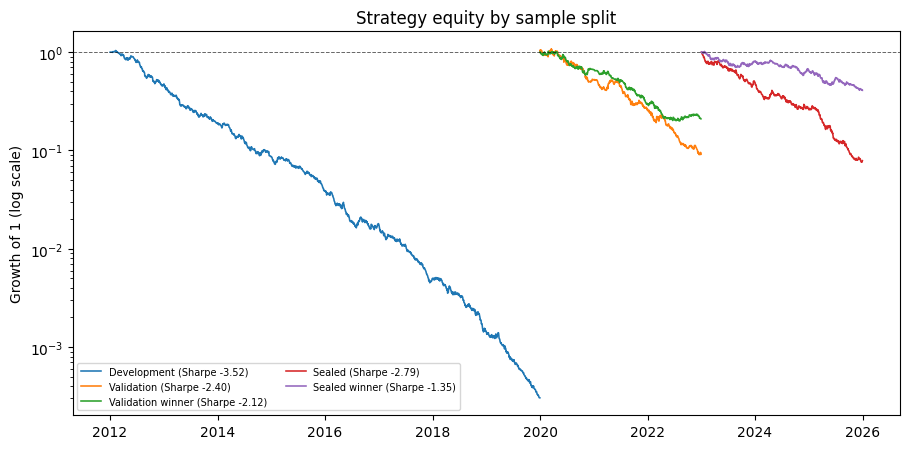
\includegraphics[width=0.92\linewidth]{figures/fig_equity.png}
\caption{Strategy equity by sample split (log scale).}
\label{fig:equity}
\end{figure}
\begin{figure}[htbp]\centering
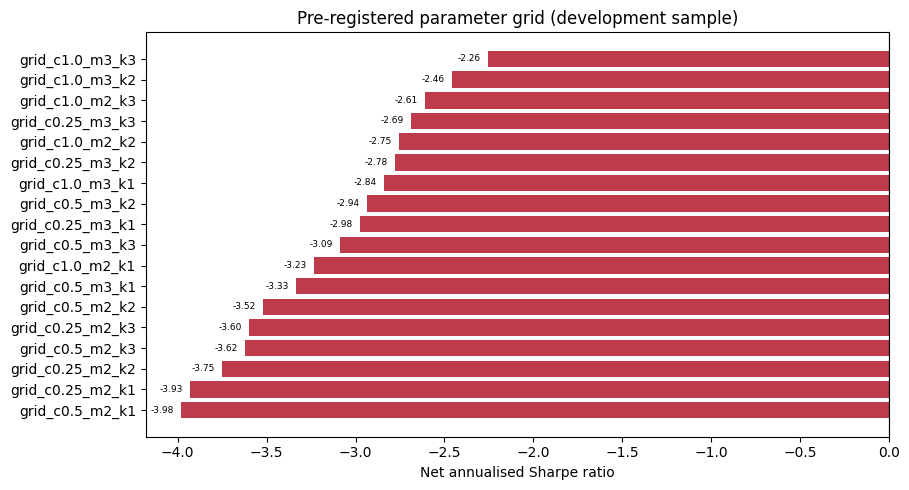
\includegraphics[width=0.92\linewidth]{figures/fig_grid.png}
\caption{Pre-registered parameter grid (development).}
\label{fig:grid}
\end{figure}
\begin{figure}[htbp]\centering
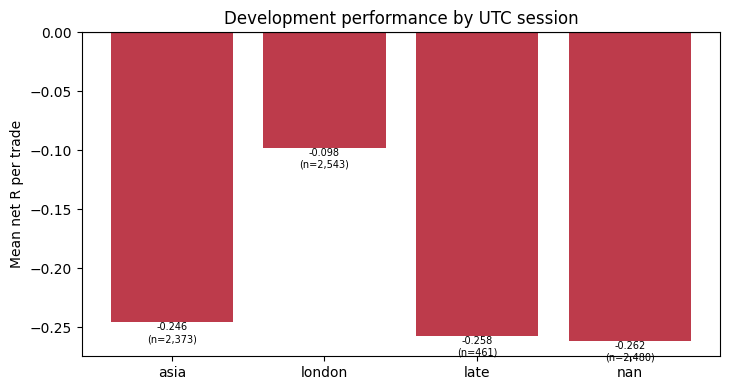
\includegraphics[width=0.92\linewidth]{figures/fig_sessions.png}
\caption{Development mean net R by UTC session.}
\label{fig:sessions}
\end{figure}
\begin{figure}[htbp]\centering
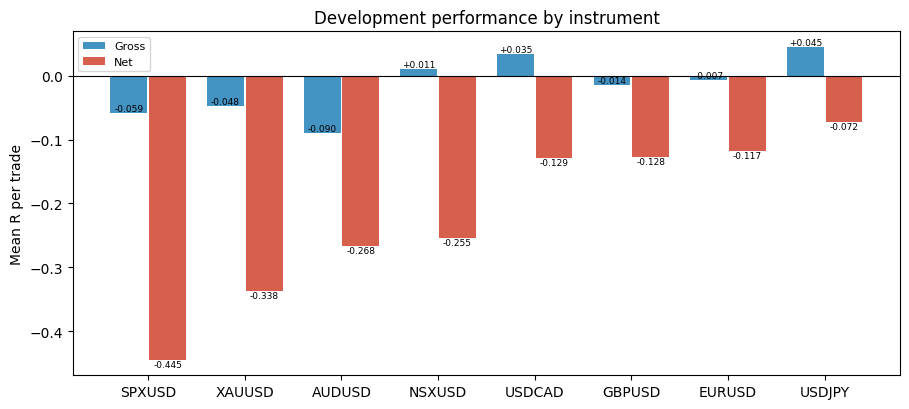
\includegraphics[width=0.92\linewidth]{figures/fig_symbols.png}
\caption{Development performance by instrument.}
\label{fig:symbols}
\end{figure}
\begin{figure}[htbp]\centering
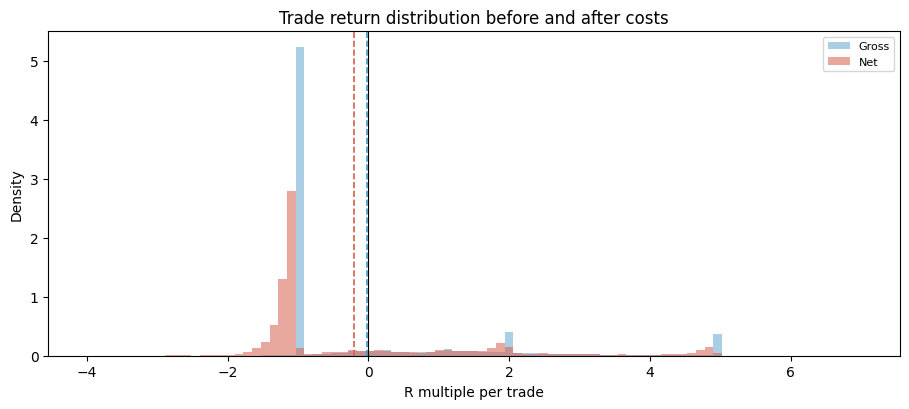
\includegraphics[width=0.92\linewidth]{figures/fig_r_distribution.png}
\caption{Trade return distribution before and after costs.}
\label{fig:rdist}
\end{figure}
\begin{figure}[htbp]\centering
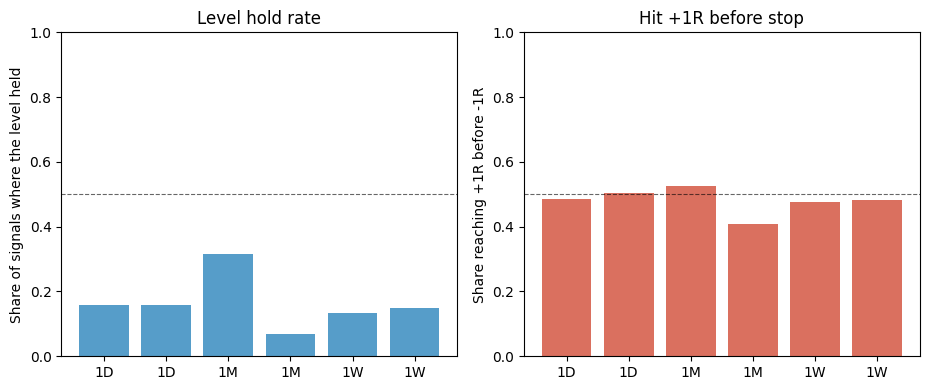
\includegraphics[width=0.92\linewidth]{figures/fig_level_reactions.png}
\caption{Level hold rate and +1R-before-stop rate.}
\label{fig:audit}
\end{figure}
\begin{figure}[htbp]\centering
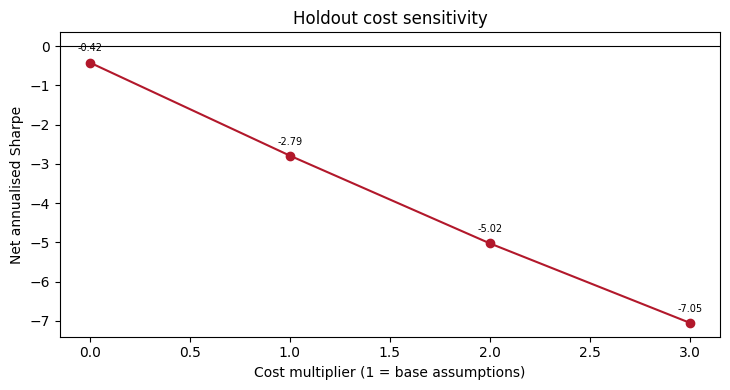
\includegraphics[width=0.92\linewidth]{figures/fig_cost_sensitivity.png}
\caption{Holdout cost sensitivity.}
\label{fig:cost}
\end{figure}
\begin{figure}[htbp]\centering
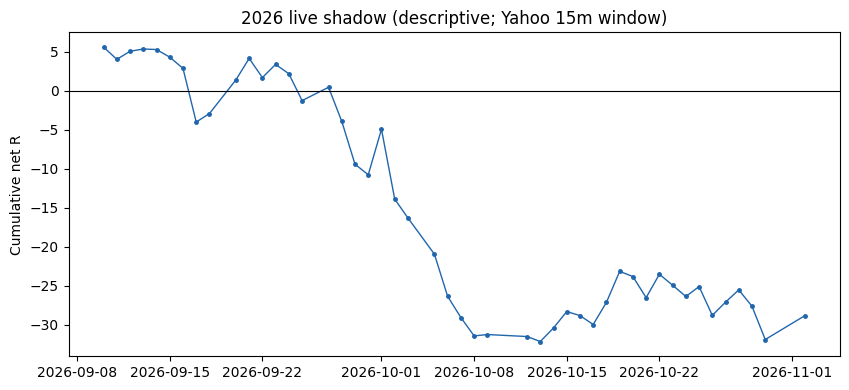
\includegraphics[width=0.92\linewidth]{figures/fig_live_shadow.png}
\caption{2026 live shadow cumulative net R.}
\label{fig:live}
\end{figure}
Table \ref{tab:benchmarks} compares the strategy with simple alternatives on the same holdout window and cost model. Buy-and-hold and the 50/200-day SMA crossover are positive; the 4-hour trend-only and Donchian benchmarks are negative. The key-level strategy is the worst of the set.
\begin{table}[htbp]
\centering
\small
\setlength{\tabcolsep}{4pt}
\caption{Holdout benchmarks on the same window and cost model.}
\label{tab:benchmarks}
\begin{tabular}{lrrrrr}
\toprule
Benchmark & Days & Annual return & Annual vol & Net Sharpe & Max DD \\
\midrule
buy\_and\_hold & 783 & 11.74\% & 5.88\% & 1.92 & -5.75\% \\
sma\_50\_200 & 783 & 3.08\% & 6.31\% & 0.51 & -5.22\% \\
trend\_only & 783 & -2.69\% & 4.13\% & -0.64 & -8.76\% \\
donchian\_20 & 783 & -2.78\% & 3.92\% & -0.70 & -8.87\% \\
\bottomrule
\end{tabular}
\end{table}
Table \ref{tab:bh} reports Benjamini--Hochberg adjusted per-instrument tests. No instrument survives false-discovery-rate control at the pre-registered alpha.
\begin{table}[htbp]
\centering
\small
\setlength{\tabcolsep}{4pt}
\caption{Per-instrument one-sided tests with Benjamini--Hochberg adjustment.}
\label{tab:bh}
\begin{tabular}{lrrr}
\toprule
Symbol & One-sided p & BH q & Reject \\
\midrule
AUDUSD & 1.0000 & 1.0000 & no \\
EURUSD & 0.9069 & 1.0000 & no \\
GBPUSD & 0.9979 & 1.0000 & no \\
NSXUSD & 0.0333 & 0.2665 & no \\
SPXUSD & 0.9549 & 1.0000 & no \\
USDCAD & 0.9998 & 1.0000 & no \\
USDJPY & 0.9909 & 1.0000 & no \\
XAUUSD & 0.7374 & 1.0000 & no \\
\bottomrule
\end{tabular}
\end{table}
\section{Discussion}
The gross edge is approximately zero before any transaction cost. This is the key economic fact: a genuine 90\% level-hold rate would earn a positive gross mean $R$ even under pessimistic path assumptions. Costs then turn a zero-mean strategy into a reliably negative one. The grid does not identify a stable profitable region, and the ablations do not reveal a hidden source of edge. The level-reaction audit separates the claim's mechanism from its profitability implication: the level holds less often than claimed, and the hold cannot be monetised after costs.
\section{Limitations}
The transcript is discretionary; the rules are a faithful but explicit translation, and a different translation could produce a different result. HistData's M1 timestamp convention is undocumented; the resampling is causal and internally consistent, but bar-open versus bar-close ambiguity remains. Spreads and slippage are stylised rather than broker quotes. The 15-minute bars cannot order the high and low, so stop-first is a lower bound; the measured ambiguity rate is small, but platform-level backtests can still differ materially because of this ambiguity \citep{claeys2026backtests}. The universe is eight instruments chosen ex ante. The live shadow is short and descriptive. No historical news calendar is used.
\section{Conclusion}
A widely taught multi-timeframe key-level strategy, operationalised deterministically and tested on 2012--2025 intraday data, does not produce a positive net edge. The gross edge is approximately zero, costs make the net result negative, every pre-registered grid point is negative, and the sealed holdout does not reverse the conclusion. The 90\% level-hold claim is not supported in this operationalisation. The result is a useful benchmark for future work on support/resistance and for the broader replication agenda in technical analysis.
\bibliographystyle{plainnat}
\bibliography{references}
\end{document}
